\documentclass[handout]{beamer}
\documentclass[compress]{beamer}
\usepackage[T1]{fontenc}
\usepackage{pifont}
\usetheme[block=fill,subsectionpage=progressbar,sectionpage=progressbar]{metropolis} 

\usepackage{minted}

\usepackage{hyperref}
\hypersetup{ %
	pdfborder = {0 0 0},
	colorlinks=true,
}



\definecolor{Purple}{HTML}{911146}
\definecolor{Orange}{HTML}{CF4A30}

% Theme colors are derived from these two elements
\setbeamercolor{alerted text}{fg=Orange}

% ... however you can of course override styles of all elements
\setbeamercolor{frametitle}{bg=Purple}


\usepackage{wasysym}
\usepackage{etoolbox}
\usepackage[utf8]{inputenc}

\usepackage{threeparttable}
\usepackage{subcaption}

\usepackage{tikz-qtree}
\setbeamercovered{still covered={\opaqueness<1->{5}},again covered={\opaqueness<1->{100}}}





\usepackage{listings}

\lstset{
	basicstyle=\scriptsize\ttfamily,
	columns=flexible,
	breaklines=true,
	numbers=left,
	%stepsize=1,
	numberstyle=\tiny,
	backgroundcolor=\color[rgb]{0.85,0.90,1}
}



\lstnewenvironment{lstlistingoutput}{\lstset{basicstyle=\footnotesize\ttfamily,
		columns=flexible,
		breaklines=true,
		numbers=left,
		%stepsize=1,
		numberstyle=\tiny,
		backgroundcolor=\color[rgb]{.7,.7,.7}}}{}


\lstnewenvironment{lstlistingoutputtiny}{\lstset{basicstyle=\tiny\ttfamily,
		columns=flexible,
		breaklines=true,
		numbers=left,
		%stepsize=1,
		numberstyle=\tiny,
		backgroundcolor=\color[rgb]{.7,.7,.7}}}{}


\usepackage[american]{babel}
\usepackage{csquotes}

\usepackage[natbib=true,style=authoryear,backend=bibtex,useprefix=true]{biblatex}
\addbibresource{../literature.bib}

%\usepackage[style=apa, backend = biber]{biblatex}
%\DeclareLanguageMapping{american}{american-UoN}
%\addbibresource{../literature.bib}
\renewcommand*{\bibfont}{\tiny}

\usepackage{tikz}
\usetikzlibrary{shapes,arrows,matrix}
\usepackage{multicol}

\usepackage{subcaption}

\usepackage{booktabs}
\usepackage{graphicx}

\graphicspath{{../pictures/}}

\makeatletter
\setbeamertemplate{headline}{%
	\begin{beamercolorbox}[colsep=1.5pt]{upper separation line head}
	\end{beamercolorbox}
	\begin{beamercolorbox}{section in head/foot}
		\vskip2pt\insertnavigation{\paperwidth}\vskip2pt
	\end{beamercolorbox}%
	\begin{beamercolorbox}[colsep=1.5pt]{lower separation line head}
	\end{beamercolorbox}
}
\makeatother



\setbeamercolor{section in head/foot}{fg=normal text.bg, bg=structure.fg}



\newcommand{\question}[1]{
	\begin{frame}[plain]
		\begin{columns}
			\column{.4\textwidth}
			\makebox[\columnwidth]{
				
\includegraphics[width=\columnwidth,height=\paperheight,keepaspectratio]{../pictures/mannetje.png}}
			\column{.6\textwidth}
			\large
			\textcolor{orange}{\textbf{\emph{#1}}}
		\end{columns}
\end{frame}}

\newcommand{\instruction}[1]{\emph{\textcolor{gray}{[#1]}}}


\title[Computational Communication Science 2]{\textbf{Computational Communication Science 2} \\Week 4 - Lecture\\ »Text similiarity and differences«}
\author[Anne Kroon]{Anne Kroon \\ ~ \\ \footnotesize{a.c.kroon@uva.nl, @annekroon} \\}
\date{April, 2022}
\institute[Digital Society Minor, University of Amsterdam]{Digital Society Minor, University of Amsterdam}


\begin{document}
	
	\begin{frame}{}
		\titlepage
	\end{frame}
	
\begin{frame}{Today}
	\tableofcontents
\end{frame}


\begin{frame}{The CCS toolbox}
	\makebox[\columnwidth]{
		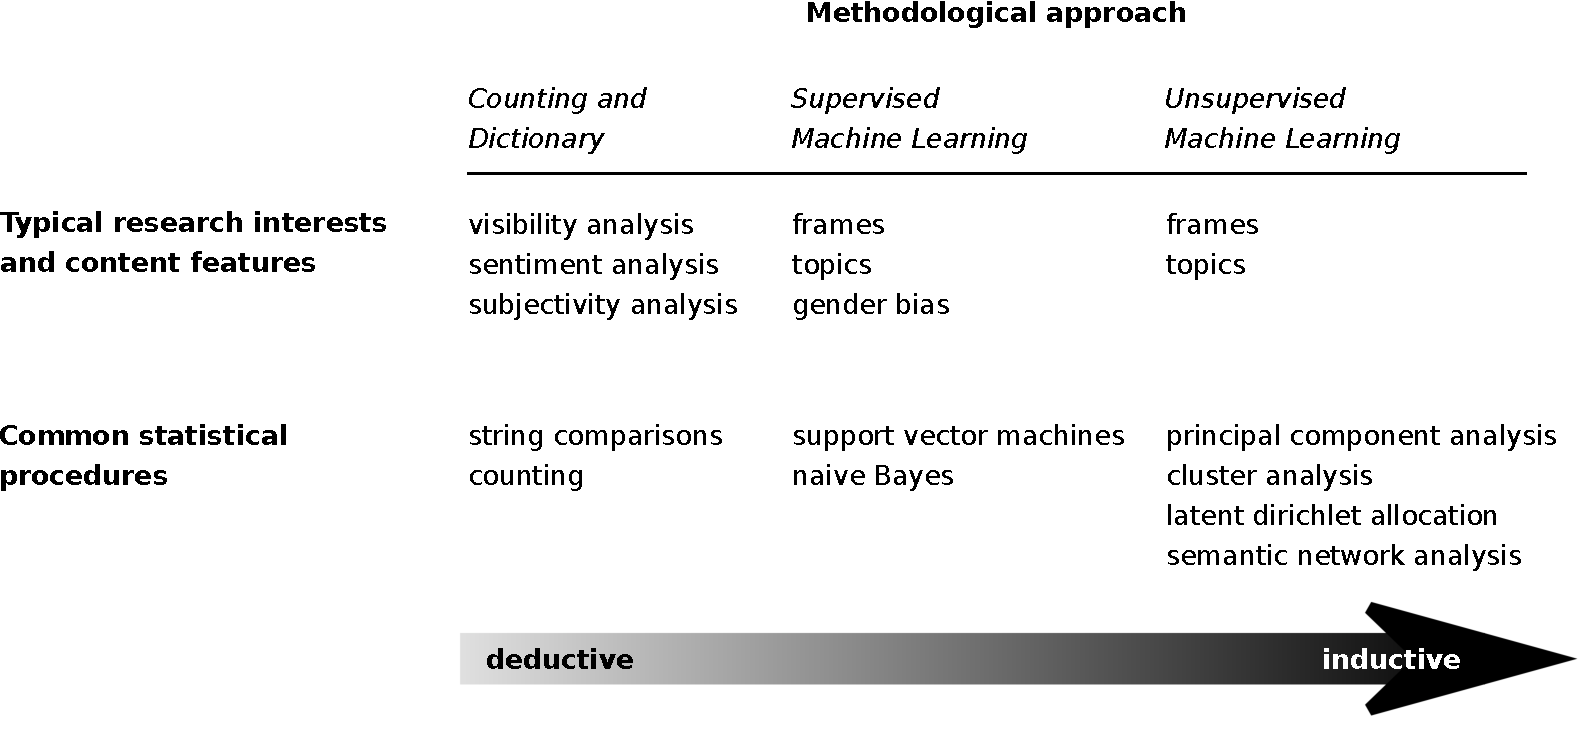
\includegraphics[width=\columnwidth,height=\paperheight,keepaspectratio]{../pictures/boumanstrilling2016}}
	\\
	\cite{Boumans2016}
\end{frame}


\section{Cosine Similarity}

\begin{frame}{Cosine Similarity}
	\begin{block}{Cosine Similarity}
		\begin{itemize}[<+>]
			\item A measure that helps you determine how similar two documents are, irrespective of their size
		\end{itemize}
	
		\begin{exampleblock}{Applications in Communication Science}
		\begin{itemize}[<+>]
			\item For example, to map \emph{linguistic alignment} of romantic couples over time \parencite{Brinberg2021}
			\item Or, in the political domain, agenda overlap between public opinion and political speech \parencite{Hager2020}
		\end{itemize}
	\end{exampleblock}
	\end{block}
\end{frame}

\begin{frame}{Cosine Similarity} 
$$
\text { similarity }=\cos (\theta)=\frac{\mathbf{A} \cdot \mathbf{B}}{\|\mathbf{A}\|\|\mathbf{B}\|}=\frac{\sum_{i=1}^{n} A_{i} B_{i}}{\sqrt{\sum_{i=1}^{n} A_{i}^{2}} \sqrt{\sum_{i=1}^{n} B_{i}^{2}}}
$$

\pause

\begin{itemize}[<+>]
\item It measures the cosine of the angle between two vectors projected in a multi-dimensional space.
\item 0 means orthogonal vectors (90 degrees); very dissimal
\item 1 means vectors are the same (0 degrees); similar
\end{itemize}
\end{frame}


\begin{frame}{Cosine Similarity}
	\makebox[\columnwidth]{
		\includegraphics[width=\columnwidth,height=\paperheight,keepaspectratio]{../pictures/cosine_angle.png}}
	\\
\footnote{https://towardsdatascience.com/what-is-cosine-similarity-how-to-compare-text-and-images-in-python-d2bb6e411ef0}
\end{frame}




% recommender systems are everywhere around us.
\begin{frame}{how can we calculate this in python?}
Let's review a practical application \footnote{https://github.com/annekroon/CCS-2/blob/main/week04/exercises/cosine-similarity-basics.ipynb}.
\end{frame}


\begin{frame}[fragile]{Implementation in Python}
	\begin{minted}[%
		breaklines,
		linenos,
		fontsize=\scriptsize,
		frame=single,
		xleftmargin=0pt,]
		{python}
from sklearn.feature_extraction.text import CountVectorizer, TfidfVectorizer
import pandas as pd

doc1 = "When I eat breakfast, I usually drink some tea".lower()
doc2 = "I like my tea with my breakfast".lower()
doc3 = "She likes cereal and coffee".lower()

vec = CountVectorizer(stop_words='english')
count_matrix = vec.fit_transform([doc1, doc2, doc3])

print(pd.DataFrame(count_matrix.A, columns=vec.get_feature_names()).to_string())
\end{minted}

\pause
%\begin{lstlistingoutput}
\begin{minted}[fontsize=\scriptsize]{python}
     breakfast  cereal  coffee  drink  eat  like  likes  tea  usually
0          1       0       0      1    1     0      0    1        1
1          1       0       0      0    0     1      0    1        0
2          0       1       1      0    0     0      1    0        0
\end{minted}
%\end{lstlistingoutput}s
\end{frame}

\begin{frame}[fragile]{Implementation in Python}
	\begin{minted}[%
		breaklines,
		linenos,
		fontsize=\scriptsize,
		frame=single,
		xleftmargin=0pt,]
		{python}
doc1_vector = pd.DataFrame(count_matrix.A, columns=vec.get_feature_names()).T[0].to_list()
doc2_vector = pd.DataFrame(count_matrix.A, columns=vec.get_feature_names()).T[1].to_list()

print(f"The vector belonging to doc1: {doc1_vector}")
print(f"The vector belonging to doc2: {doc2_vector}")
	\end{minted}
	
	\pause
	%\begin{lstlistingoutput}
	\begin{minted}{python}
The vector belonging to doc1: [1, 0, 0, 1, 1, 0, 0, 1, 1]
The vector belonging to doc2: [1, 0, 0, 0, 0, 1, 0, 1, 0]
	\end{minted}
	%\end{lstlistingoutput}s
\end{frame}


\begin{frame}[fragile]{Implementation in Python}
Now, lets populate the formula.
1.Execute the part of the formula in the numerator. Specifically, take the dot product of the vectors:
$$
\sum_{i=1}^{n} A_{i} B_{i}
$$

\begin{minted}[fontsize=\scriptsize]{python}
doc1: [1, 0, 0, 1, 1, 0, 0, 1, 1]
doc2: [1, 0, 0, 0, 0, 1, 0, 1, 0]
\end{minted}
%\end{lstlistingoutput}s
$$
dot\_product = (1\cdot1) + (0\cdot0) + (0\cdot0) + (1\cdot0) + (1\cdot0) + (0\cdot0) + (1\cdot1) +(1\cdot0)
$$
\pause
Or, using Python: 
	\begin{minted}[%
		breaklines,
		linenos,
		fontsize=\scriptsize,
		frame=single,
		xleftmargin=0pt,]
		{python}
dot_product = sum([num1 * num2 for num1, num2 in zip(doc1_vector, doc2_vector)])
print(dot_product)
	\end{minted}
\pause
	%\begin{lstlistingoutput}
	\begin{minted}{python}
2
	\end{minted}
	%\end{lstlistingoutput}s
\end{frame}



\begin{frame}[fragile]{Implementation in Python}
    2.Execute the part of the formula in the denumerator. Take the cross product of the two vectors.

$$
\sqrt{\sum_{i=1}^{n} A_{i}^{2}} \sqrt{\sum_{i=1}^{n} B_{i}^{2}}
$$
\footnotesize{Calculate this by hand:
$$
doc1_ = \sqrt{1^2 + 0^2 + 0^2 + 1^2 + 1^2 + 0^2+ 1^2 + 1^2}
$$
$$
doc1_ = \sqrt{1^2 + 0^2 + 0^2 + 0^2 + 1^2 + 0^2+ 1^2 + 0^2}
$$
}
\pause
Implementation in Python:
	\begin{minted}[%
		breaklines,
		linenos,
		fontsize=\scriptsize,
		frame=single,
		xleftmargin=0pt,]
		{python}
import math
doc1_ = math.sqrt(sum( [i**2 for i in doc1_vector]) )
doc2_ = math.sqrt(sum( [i**2 for i in doc2_vector]) )

doc1_ * doc2_
\end{minted}
	\pause
%\begin{lstlistingoutput}
\begin{minted}{python}
3.872983346207417
\end{minted}
%\end{lstlistingoutput}s
\end{frame}


\begin{frame}[fragile]{Implementation in Python}
	3.Finally:

\begin{minted}[%
	breaklines,
	linenos,
	fontsize=\scriptsize,
	frame=single,
	xleftmargin=0pt,]
	{python}
cos_sim = dot_product / (doc1_ * doc2_)
print(cos_sim)
\end{minted}

\pause

\begin{minted}[fontsize=\scriptsize]{python}
0.5163977794943222
\end{minted}
\end{frame}

\begin{frame}[fragile]{Implementation in Python}

We can, however, do this much faster using sklearn's \texttt{cosine\_similarity}.
	
\begin{minted}[%
	breaklines,
	linenos,
	fontsize=\scriptsize,
	frame=single,
	xleftmargin=0pt,]
	{python}
from sklearn.metrics.pairwise import cosine_similarity
cosine_similarity([doc1_vector, doc2_vector])
\end{minted}
	
	\pause
	
\begin{minted}[fontsize=\scriptsize]{python}
array([[1.        , 0.51639778],
[0.51639778, 1.        ]])
	\end{minted}
\end{frame}

\begin{frame}{How to use this in practice}
	\begin{block}{What can you do with this?}
		\begin{itemize}[<+>]
			\item This is especially powerful if you want to compare different news articles, movies, song texts, etc.
			\item For example, which movies are most similair in terms of genre composition?
			\end{itemize}
	\end{block}
\end{frame}

\begin{frame}
	\makebox[\linewidth]{
		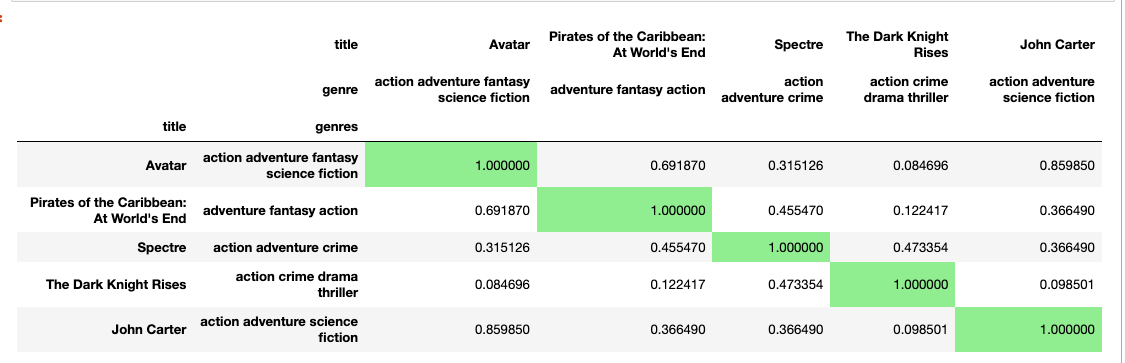
\includegraphics[width=\columnwidth,height=\paperheight,keepaspectratio]{../pictures/cosine_sim.png}}
Indentify movies that are similar in terms of genre  \footnote{https://www.learndatasci.com/glossary/cosine-similarity/}
\end{frame}

\begin{frame}{Considering Cosine Similarity}
	\begin{block}{Things to consider}
		\begin{itemize}
		\item <1-> What type of overlap are you interested in?
		\item <2->What is the meaning of n-grams, stems,  stopwords when considering your RQ? How you should preproces, depends on your RQ and aim. 
		\item <3-> Computationally cheap and fast; works well in e.g., recommender systems (week 6!)
		\end{itemize}
	\end{block}
\begin{alertblock}{Drawbacks}
	\begin{itemize}
	\item <4-> An \emph{exact} match in terms of words is needed. Is that realistic?	
	\end{itemize}
\end{alertblock}
\end{frame}

\begin{frame}[fragile]{Implementation in Python}
	\begin{minted}[%
		breaklines,
		linenos,
		fontsize=\scriptsize,
		frame=single,
		xleftmargin=0pt,]
		{python}
doc1 = "When I eat breakfast, I usually drink some tea".lower()
doc2 = "I like my tea with my breakfast".lower()
doc3 = "She likes cereal and coffee".lower()
	\end{minted}
	What do you expect here? Should there be some level of overlap?
\end{frame}


\begin{frame}[fragile]{Implementation in Python}
\begin{minted}[%
	breaklines,
	linenos,
	fontsize=\scriptsize,
	frame=single,
	xleftmargin=0pt,]
	{python}
doc1 = "When I eat breakfast, I usually drink some tea".lower()
doc2 = "I like my tea with my breakfast".lower()
doc3 = "She likes cereal and coffee".lower()
\end{minted}
	
\begin{minted}[%
	breaklines,
	linenos,
	fontsize=\scriptsize,
	frame=single,
	xleftmargin=0pt,]
	{python}
print(cosine_similarity([doc1_vector, doc2_vector, doc3_vector]))
\end{minted}
	\pause
\begin{minted}[fontsize=\scriptsize]{python}
[[1.         0.51639778 0.        ]
[0.51639778 1.         0.        ]
[0.         0.         1.        ]]
\end{minted}
	\pause
Zero overlap between doc3 and the other documents. Is that correct?
\end{frame}


\section{Soft cosine similarity}
\begin{frame}{Soft cosine similarity}
	\huge{...enter soft cosine similarty} \parencite{Sidorov2014}\\
	\pause
	\footnotesize{``Soft Cosine Measure (SCM) is a method that allows us to assess the similarity between two documents in a meaningful way, even when they have no words in common. It uses a measure of similarity between words, which can be derived using [word2vec] vector embeddings of words.''}
	\footnote{\url{https://radimrehurek.com/gensim//auto_examples/tutorials/run_scm.html}}
\end{frame}

\begin{frame}{Soft Cosine Measure (SCM)}
	\begin{block}{SCM}
		\begin{itemize}
			\item <1-> Even if two sentences do not share the same words, we can calculate similarity by modelling \emph{synonym}
			\item <2->For example, the words `play' and `game' are different but related \parencite{Sidorov2014} \footnote{\url{http://www.scielo.org.mx/pdf/cys/v18n3/v18n3a7.pdf}}
			\item<3->How can we capture `semantic' meaning?
		\end{itemize}
	\end{block}
	\begin{exampleblock}{How?}
		\begin{itemize}
			\item <4-> Convert words to \emph{word vectors} and then compute similarities  \footnote{\url{https://www.machinelearningplus.com/nlp/cosine-similarity/}}
		\end{itemize}
	\end{exampleblock}
\end{frame}


\begin{frame}
	\makebox[\linewidth]{
		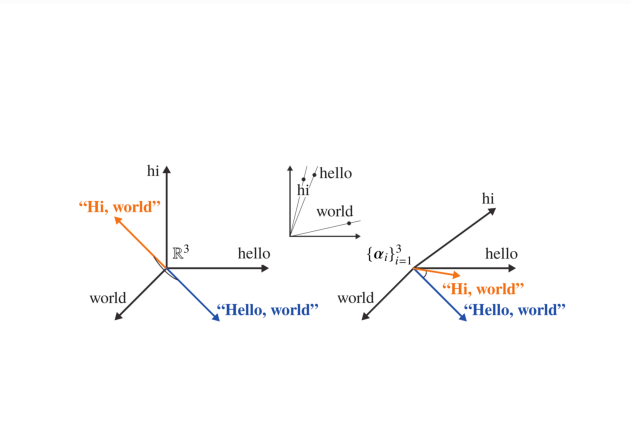
\includegraphics[width=\columnwidth,height=\paperheight,keepaspectratio]{../pictures/soft-cosine}}
	Soft cosine similarity \footnote{\url{https://radimrehurek.com/gensim//auto_examples/tutorials/run_scm.html}}
\end{frame}

\begin{frame}{Word embeddings}
	\begin{block}{Word embeddings}
		\begin{itemize}
			\item <1->To use the SCM, you need word embeddings. 
		\end{itemize}
	\end{block}
\end{frame}

\subsection{Word embeddings}

\begin{frame}{Understanding SCM}
SCM estimates extracts similarity from \alert{word embeddings}. 
	\begin{block}{What are word embeddings?}
		\begin{itemize}[<+>]
			\item No technical details here, just the general idea
			\item Word embeddings help capturing the meaning of text
			\item Word embeddings are low-dimensional vector representations that capture semantic meaning
			\item State-of-the-art in NLP...
			\item \emph{``...a word is characterized by the company it keeps...''} (Firth, 1957)
		\end{itemize}
	\end{block}
\end{frame}

\iffalse
\begin{frame}{}
	\makebox[\linewidth]{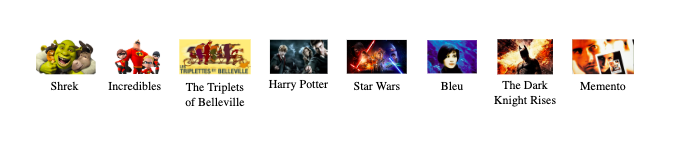
\includegraphics[width=\linewidth,height=\textheight, keepaspectratio]{../pictures/google1.png}}
\end{frame}

\begin{frame}{}
	\makebox[\linewidth]{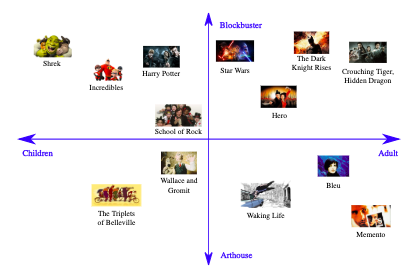
\includegraphics[width=\linewidth,height=\textheight, keepaspectratio]{../pictures/google2.png}}
\end{frame}


\begin{frame}{}
	\makebox[\linewidth]{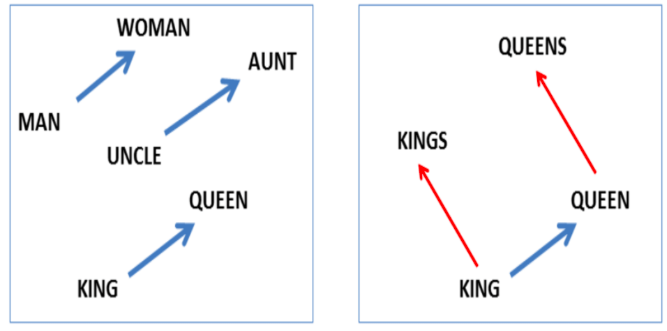
\includegraphics[width=\linewidth,height=\textheight, keepaspectratio]{../pictures/embeddings.png}}
	
	$king-man+woman = ?$ 
\end{frame}


\begin{frame}{}
	\makebox[\linewidth]{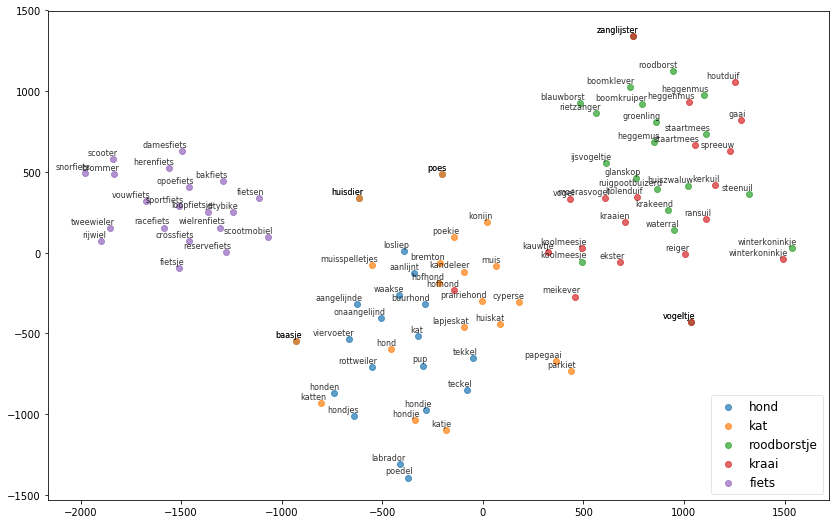
\includegraphics[width=\linewidth,height=\textheight, keepaspectratio]{../pictures/w2v_300_illustration.png}}
\end{frame}


\begin{frame}{}
	\makebox[\linewidth]{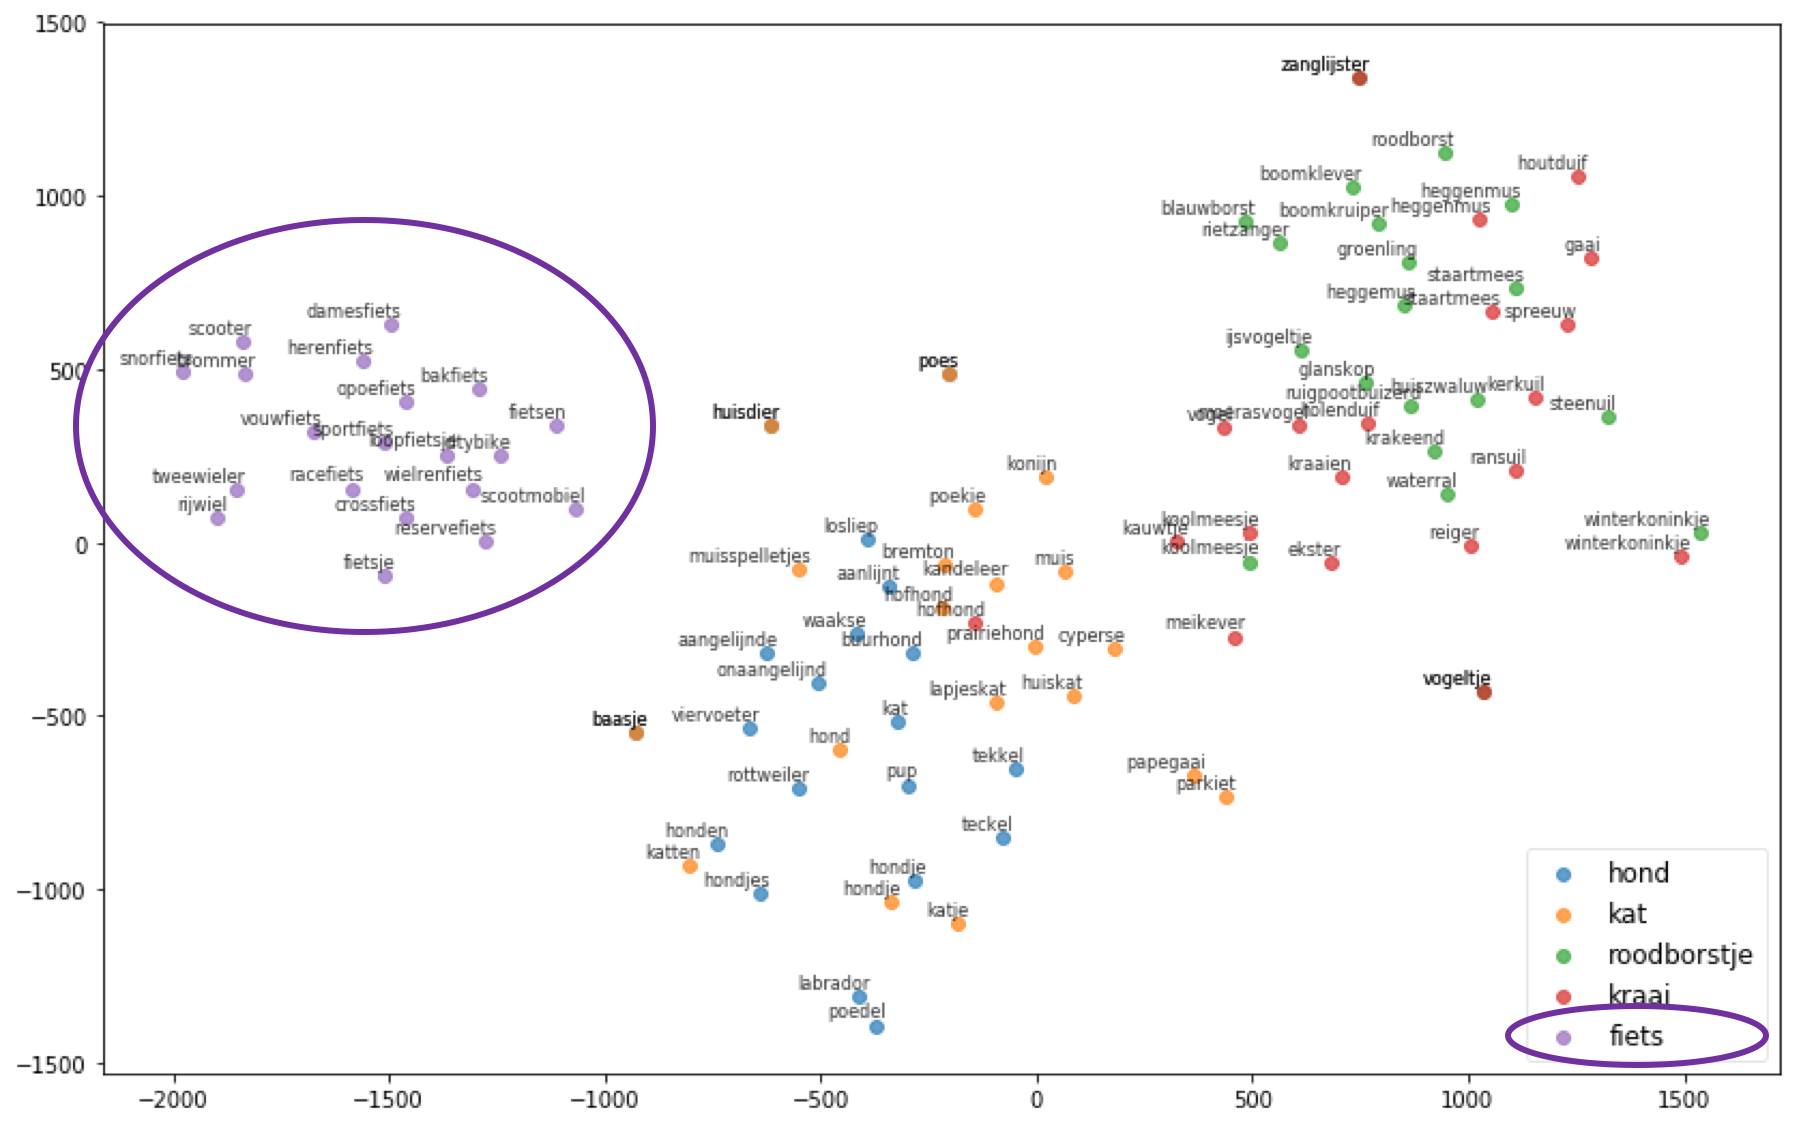
\includegraphics[width=\linewidth,height=\textheight, keepaspectratio]{../pictures/visual2.png}}
\end{frame}

%as can be seen, words most similar to fiets are on the left. 

\begin{frame}{}
	\makebox[\linewidth]{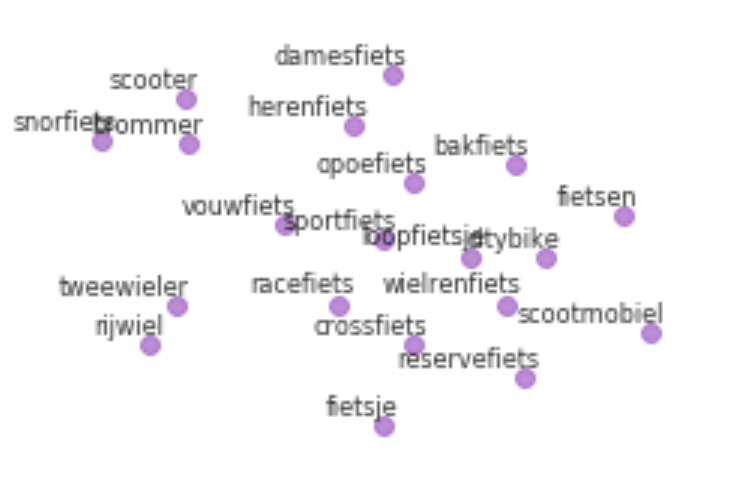
\includegraphics[width=\linewidth,height=\textheight, keepaspectratio]{../pictures/fiets}}
\end{frame}

%the model has learned that fiets is similar to racefiets, wielrenfiets, rijwiel - and different from the animal department: it doesnt overlap with our kats/ dogs and birds clusters

\begin{frame}{}
	\makebox[\linewidth]{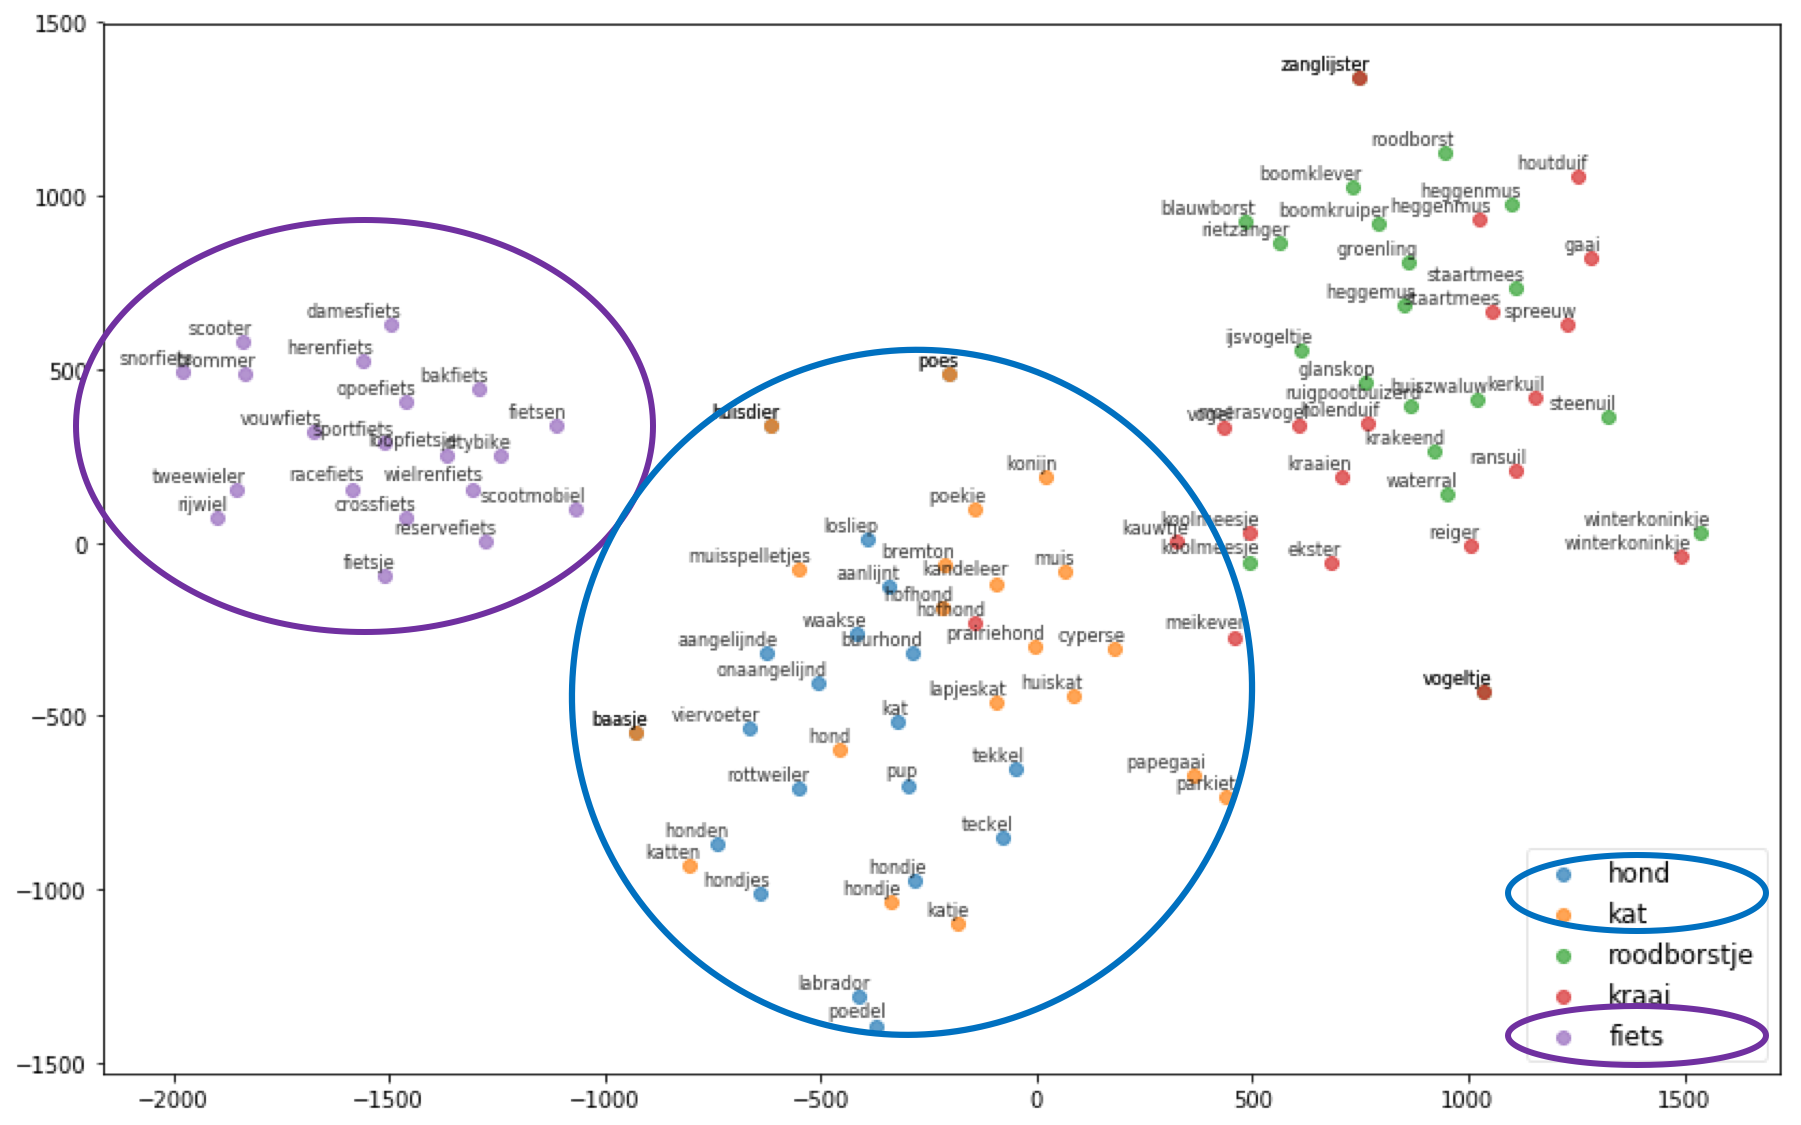
\includegraphics[width=\linewidth,height=\textheight, keepaspectratio]{../pictures/visual1.png}}
\end{frame}

%the model recognizes that fiets is something else from honden and katten. Both mammals and pets, dogs and cats are quite similar and appear in the same cluster.  

\begin{frame}{}
	\makebox[\linewidth]{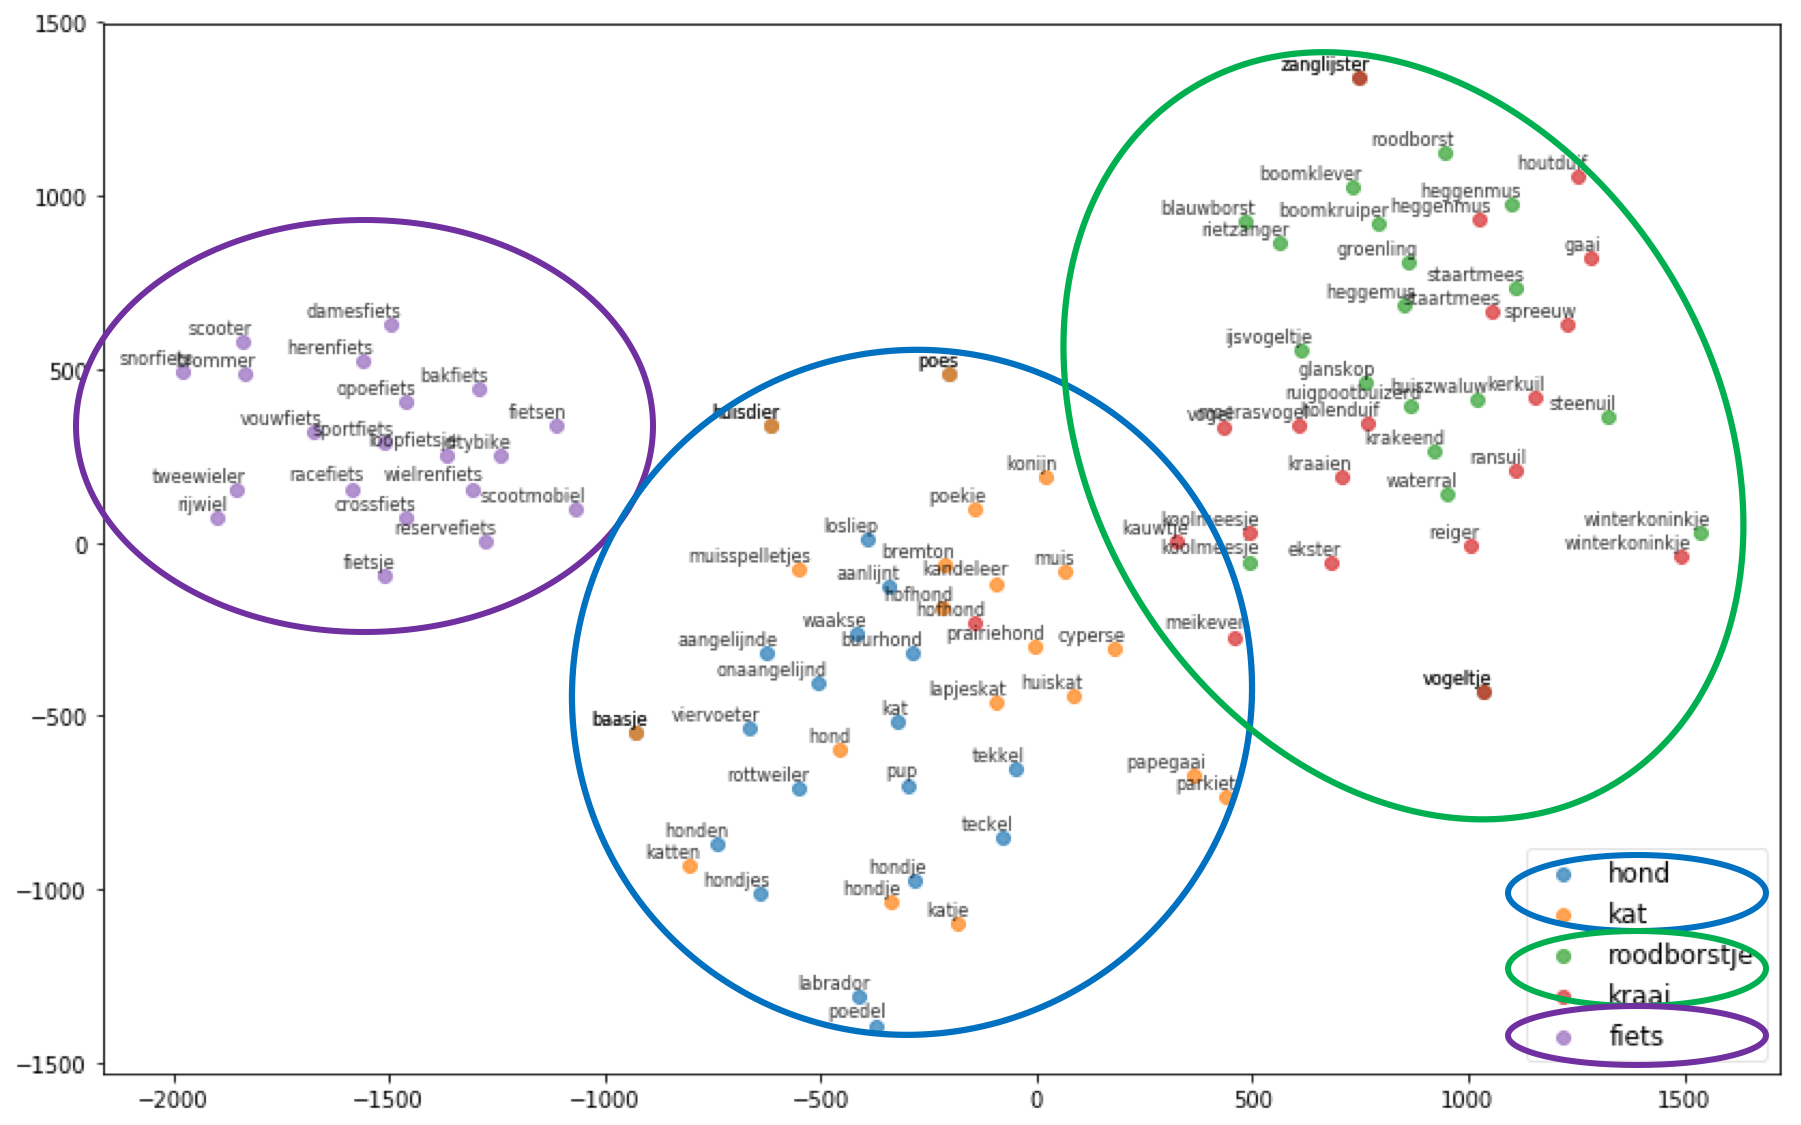
\includegraphics[width=\linewidth,height=\textheight, keepaspectratio]{../pictures/visual.png}}
\end{frame}
\fi



\subsection{Implemention in Python}
\begin{frame}[fragile]{SCM in Python}
	\begin{block}{Calculating Soft Cosine Measure}
		\begin{itemize}
			\item<1->To use the SCM, you need embeddings. 
			\item<2-> We \emph{can} train embeddings on our own corpus (if we had a lot of data) \dots
			\item<3-> But for now we will use pre-trained models \footnote{\url{https://github.com/annekroon/CCS-2/blob/main/week04/exercises/cosine-similarity-basics.ipynb}}. \dots
		\end{itemize}
	\end{block}
\pause
\pause
\pause
\begin{minted}[%
	breaklines,
	fontsize=\scriptsize,
	frame=single,
	xleftmargin=0pt,]
	{python}
import gensim.downloader as api
	
fasttext_model300 = api.load('fasttext-wiki-news-subwords-300')
\end{minted}
\end{frame}

\begin{frame}[fragile]{Create a dictionary}	
\footnotesize{Let's review our 3 documents:}
\begin{minted}[%
breaklines,
linenos,
fontsize=\tiny,
frame=single,
xleftmargin=0pt,]
	{python}
doc1 = "When I eat breakfast, I usually drink some tea".lower()
doc2 = "I like my tea with my breakfast".lower()
doc3 = "She likes cereal and coffee".lower()	
\end{minted}
\pause
\footnotesize{Initialize a Dictionary. This step assigns a \texttt{token\_id} to each word:}
\begin{minted}[%
breaklines,
linenos,
fontsize=\tiny,
frame=single,
xleftmargin=0pt,]
{python}
from gensim.utils import simple_preprocess
from gensim.corpora import Dictionary
dictionary = corpora.Dictionary([simple_preprocess(doc) for doc in [doc1, doc2, doc3]]) 
\end{minted}
\pause
\footnotesize{Now, let's check whether a specific word--for example \texttt{coffee}--is in our \texttt{dictionary:}}
\begin{minted}[%
breaklines,
linenos,
fontsize=\tiny,
frame=single,
xleftmargin=0pt,]
	{python}
'coffee' in dictionary.token2id
\end{minted}
	\pause
	%\begin{lstlistingoutput}
	\begin{minted}{python}
True
	\end{minted}
\end{frame}


\begin{frame}[fragile]{Create a bag-of-words representation}	
\footnotesize{Next, let's represent each document by \texttt{(token\_id, token\_count)} tuples}:
\begin{minted}[%
breaklines,
linenos,
fontsize=\scriptsize,
frame=single,
xleftmargin=0pt,]
{python}
bag_of_words_vectors = [ dictionary.doc2bow(simple_preprocess(doc)) for doc in [doc1, doc2, doc3]] 
\end{minted}
\pause
\footnotesize{Build a term similarity matrix and compute a sparse term similarity matrix}:
\begin{minted}[%
	breaklines,
	linenos,
	fontsize=\scriptsize,
	frame=single,
	xleftmargin=0pt,]
	{python}
from gensim.similarities import SparseTermSimilarityMatrix
from gensim.similarities import WordEmbeddingSimilarityIndex

similarity_index = WordEmbeddingSimilarityIndex(fasttext_model300)
similarity_matrix = SparseTermSimilarityMatrix(similarity_index, dictionary)
\end{minted}
\end{frame}

\begin{frame}[fragile]{Inspect results}	
	\footnotesize{Get SCM using \texttt{.inner\_product()}: }:
	\begin{minted}[%
		breaklines,
		linenos,
		fontsize=\tiny,
		frame=single,
		xleftmargin=0pt,]
		{python}
#between doc1 and doc2:
scm_doc1_doc2 = similarity_matrix.inner_product(bag_of_words_vectors[0], bag_of_words_vectors[1], normalized=(True, True))

#between doc1 and doc3:
scm_doc1_doc3 = similarity_matrix.inner_product(bag_of_words_vectors[0], bag_of_words_vectors[2], normalized=(True, True))

#between doc2 and doc3;
scm_doc2_doc3 = similarity_matrix.inner_product(bag_of_words_vectors[1], bag_of_words_vectors[2], normalized=(True, True))

print(f"SCM between:\ndoc1 <-> doc2: {scm_doc1_doc2:.2f}\ndoc1 <-> doc3: {scm_doc1_doc3:.2f}\ndoc2 <-> doc3: {scm_doc2_doc3:.2f}")
	\end{minted}
	\pause
	\footnotesize{Do the results make more sense?}:
	\begin{minted}[%
		fontsize=\tiny,]
		{python}
SCM between:
doc1 <-> doc2: 0.29
doc1 <-> doc3: 0.15
doc2 <-> doc3: 0.28
\end{minted}
\end{frame}
	
\begin{frame}{Applications of cosine and soft cosine similarity}
	Applications of \emph{cosine} and \emph{soft cosine} in the field of Communication Science generally involve some overtime dynamics. 
	\begin{exampleblock}{Trace convergence or agenda setting dynamics over time}
		\begin{itemize}
			\item Beyond the scope this course to discuss it here, but if you are interested in how you can apply cosine and soft cosine in an overtime analysis, we have prepared a notebook that will help you do just that. 
			\item \url{https://github.com/annekroon/CCS-2/blob/main/week04/exercises/OPTIONAL_overtime_similarity.ipynb}
		\end{itemize}
	\end{exampleblock}

\end{frame}

\section{Topic modelling}

\begin{frame}{Let's assume you want to know a bit more about the \emph{content} you are investigating}
Cosine and soft cosine do \emph{not} inform us about substantive issues present in text. 
	\begin{enumerate}
		\item Which topics can we extract from the corpus?
		\item How present is each of these topics in each text in the corpus?
	\end{enumerate}
\end{frame}

\begin{frame}[fragile]{Recap: Document-term matrix}
	Document-term matrix
	\begin{lstlisting}
      w1,w2,w3,w4,w5,w6 ...
text1, 2, 0, 0, 1, 2, 3 ...
text2, 0, 0, 1, 2, 3, 4 ...
text3, 9, 0, 1, 1, 0, 0 ...
...
	\end{lstlisting}
	{\small{These can be simple counts, but also more advanced metrics, like tf-idf scores (where you weigh the frequency by the number of documents in which it occurs), cosine distances, etc.}}
	\pause
	\begin{itemize}
		\item given a term-document matrix, easy to do with any tool
		\item probably extremely skewed distributions
	\end{itemize}
	
\end{frame}


\begin{frame}{Recap: clustering}
	\begin{itemize}
		\item given a term-document matrix, we can easily find clusters of documents that resemble each other
	\end{itemize}
\end{frame}


\begin{frame}{We need other models to}
	\begin{enumerate}[<+->]
		\item model \emph{simultaneously} (a) which topics we find in the whole corpus, and (b) which of these topics are present in which document; while at the same time
		\item allowing (a) words to be part of multiple topics, and (b) multiple topics to be present in one document; and
		\item being able to make connections between words ``even if they never actually occured in a document together'' \parencite{Maier2018}[p.~96]
	\end{enumerate}
	
	\tiny{Maier, D., Waldherr, A., Miltner, P., Wiedemann, G., Niekler, A., Keinert, A., \ldots Adam, S. (2018). Applying LDA Topic Modeling in Communication Research: Toward a Valid and Reliable Methodology. \textit{Communication Methods and Measures, 12}(2--3), 93--118. doi:10.1080/19312458.2018.1430754}
\end{frame}


\subsection{An introduction to LDA}

\begin{frame}{}
	Enter \textbf{topic modeling with Latent Dirichlet Allocation (LDA)}
\end{frame}


\begin{frame}{LDA, what's that?}
	\begin{block}{No mathematical details here, but the general idea}
		\begin{itemize}
			\item There are $k$ topics, $T_1$\ldots$T_k$
			\item Each document $D_i$ consists of a mixture of these topics, e.g.$80\% T_1, 15\% T_2, 0\% T_3, \ldots 5\% T_k $
			\item On the next level, each topic consists of a specific probability distribution of words
			\item Thus, based on the frequencies of words in $D_i$, one can infer its distribution of topics
			\item Note that LDA is a Bag-of-Words (BOW) approach
		\end{itemize}
	\end{block}
	
\end{frame}


\begin{frame}[fragile]{Doing a LDA in Python}
We will use gensim \parencite{Rehurek10softwareframework} for this (make sure you have version >4.0)
	
Let us assume you have a list of lists of documents called \texttt{texts}:
\begin{minted}[%
	breaklines,
	linenos,
	fontsize=\tiny,
	frame=single,
	xleftmargin=0pt,]
	{python}
print(texts[0][:115])
\end{minted}
\pause
which looks something like:
\begin{minted}[%
	fontsize=\tiny,
	breaklines,]
	{python}
'Stop the presses: CNN covered some actual news yesterday when it reported on the story of medical kidnapping victim Alyssa Gilderhus at the Mayo Clinic. But was it actually InfoWars and FreeMartyG which publicly shamed CNN into doing this real journalism? Cue the Mission Impossible theme music for this one...\n\nThis mission, as we accepted it, began more than a year ago during the baby Charlie Gard medical kidnapping scandal in the UK and we thought that it had ended with an apparently unsuccessf'
\end{minted}
	
	\tiny{{\v R}eh{\r u}{\v r}ek, R., \& Sojka, P. (2010). Software framework for topic modelling with large corpora. \emph{Proceedings of the LREC 2010 Workshop on New Challenges for NLP Frameworks}, pp. 45–50. Valletta, Malta: ELRA. }
\end{frame}

\begin{frame}[fragile]{Preprocessing}
Your preprocessing steps and feature engineering decisions \emph{largely} affect your topics
	\begin{enumerate}
		\item<1-> You can apply 'manual' preprocessing steps \dots
		\item<2->\dots In isolation or combination with for example \texttt{tfidf} transformations
	\end{enumerate}
\pause
\pause
\begin{minted}[%
breaklines,
linenos,
fontsize=\tiny,
frame=single,
xleftmargin=0pt,]
{python}
texts_clean = [text.lower() for text in texts]
texts_clean=[" ".join(text.split()) for text in texts_clean]  #remove dubble spaces
texts_clean = ["".join([l for l in text if l not in punctuation]) for text in texts_clean] #remove punctuaction
texts_clean[0][:500]
\end{minted}
\pause
which looks something like:
\begin{minted}[%
breaklines,
fontsize=\tiny,]
{python}
'stop the presses cnn covered some actual news yesterday when it reported on the story of medical kidnapping victim alyssa gilderhus at the mayo clinic but was it actually infowars and freemartyg which publicly shamed cnn into doing this real journalism cue the mission impossible theme music for this one this mission as we accepted it began more than a year ago during the baby charlie gard medical kidnapping scandal in the uk and we thought that it had ended with an apparently unsuccessful april '
\end{minted}
\end{frame}


\begin{frame}[fragile]{Preprocessing}
Without \emph{stopword removal},  \emph{tfidf} transformation and/or \emph{pruning}, you topics will not be very informative.
\pause
	\begin{minted}[%
		breaklines,
		linenos,
		fontsize=\tiny,
		frame=single,
		xleftmargin=0pt,]
		{python}
mystopwords = set(stopwords.words('english')) # use default NLTK stopword list; alternatively:
# mystopwords = set(open('mystopwordfile.txt').readlines())  #read stopword list from a textfile with one stopword per line
texts_clean = [" ".join(word for word in text.split() if word not in mystopwords) for text in texts_clean]
texts_clean[0][:500]
	\end{minted}
	\pause
	which looks something like:
	\begin{minted}[%
		breaklines,
		fontsize=\tiny,]
		{python}
'stop presses cnn covered actual news yesterday reported story medical kidnapping victim alyssa gilderhus mayo clinic actually infowars freemartyg publicly shamed cnn real journalism cue mission impossible theme music one mission accepted began year ago baby charlie gard medical kidnapping scandal uk thought ended apparently unsuccessful april fools joke cnn sure many recall charlie gard infant rare form otherwise notsorare condition mitochondrial disease story went viral made international news '
	\end{minted}
\end{frame}

\begin{frame}[fragile]{Tokenization}
\texttt{gensim} expects a list of words (hence: \texttt{tokenize} your corpus)
	\pause
\begin{minted}[%
		breaklines,
		linenos,
		fontsize=\tiny,
		frame=single,
		xleftmargin=0pt,]
		{python}
tokenized_texts_clean = [TreebankWordTokenizer().tokenize(text) for text in texts_clean ] # tokenize texts; convert all strings to a list of tokens
tokenized_texts_clean[0][:500]
	\end{minted}
	\pause
	which looks something like:
	\begin{minted}[%
		breaklines,
		fontsize=\tiny,]
		{python}
['stop',
'presses',
'cnn',
'covered',
'actual',
'news',
'yesterday',
'reported',
'story',
..
	\end{minted}
\end{frame}

\begin{frame}[fragile]{LDA implementation}
	\texttt{LDA} implementation
	\pause
	\begin{minted}[%
		breaklines,
		linenos,
		fontsize=\tiny,
		frame=single,
		xleftmargin=0pt,]
		{python}
raw_m1 = tokenized_texts_clean

# assign a token_id to each word
id2word_m1 = corpora.Dictionary(raw_m1)   
# represent each text by (token_id, token_count) tuples
ldacorpus_m1 = [id2word_m1.doc2bow(text) for text in raw_m1] 

#estimate the model
lda_m1 = models.LdaModel(ldacorpus_m1, id2word=id2word_m1, num_topics=10)
lda_m1.print_topics()
	\end{minted}
	\pause

\begin{minted}[%
		breaklines,
		fontsize=\tiny,]
		{python}
[(0,
'0.015*"trump" + 0.012*"said" + 0.006*"president" + 0.006*"people" + 0.004*"cnn" + 0.004*"us" + 0.004*"house" + 0.004*"news" + 0.003*"also" + 0.003*"twitter"'),
(1,
'0.010*"said" + 0.008*"trump" + 0.004*"one" + 0.004*"people" + 0.004*"us" + 0.004*"president" + 0.004*"would" + 0.003*"media" + 0.003*"also" + 0.003*"new"'),
(2,
'0.011*"trump" + 0.009*"said" + 0.007*"president" + 0.005*"would" + 0.004*"people" + 0.004*"us" + 0.003*"also" + 0.003*"like" + 0.003*"news" + 0.003*"state"'),
(3,
'0.010*"trump" + 0.006*"president" + 0.005*"said" + 0.004*"would" + 0.004*"us" + 0.003*"also" + 0.003*"people" + 0.003*"media" + 0.003*"news" + 0.003*"one"'),
\end{minted}
\end{frame}




\begin{frame}[fragile]{Visualization with pyldavis}
	\begin{minted}[%
	breaklines,
	linenos,
	fontsize=\tiny,
	frame=single,
	xleftmargin=0pt,]
	{python}
import pyLDAvis
import pyLDAvis.gensim_models as gensimvis
# first estiate gensim model, then:
vis_data = gensimvis.prepare(lda_m1,ldacorpus_m1,id2word_m1)
pyLDAvis.display(vis_data)
\end{minted}
	\makebox[\linewidth]{
		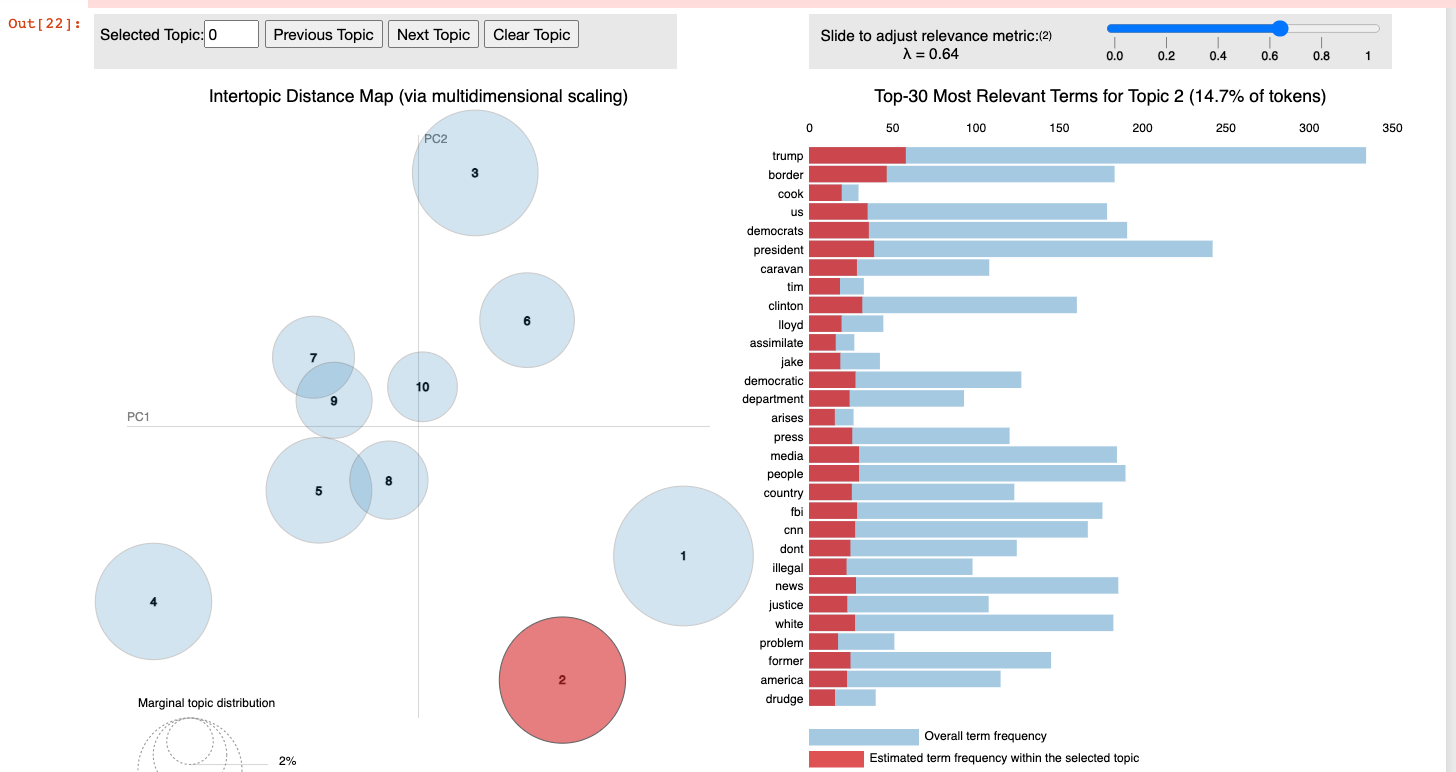
\includegraphics[width=\paperwidth,height=.5\paperheight,keepaspectratio]{../pictures/lda}}
\end{frame}

\iffalse
\begin{frame}{Visualization with pyldavis}
	Short note about the $\lambda$ setting:
	
	It influences the ordering of the words in pyldavis.
	
	\begin{quote}
		``For $\lambda = 1$, the ordering of the top words is equal to the ordering of the standard conditional word probabilities. For $\lambda$ close to zero, the most specific words of the topic will lead the list of top words. In their case study, Sievert and Shirley (2014, p. 67) found the best interpretability of topics using a  $\lambda$-value close to .6, which we adopted for our own case'' (Maier et al., 2018, p.~107)
	\end{quote}
	
	
	\tiny{Maier, D., Waldherr, A., Miltner, P., Wiedemann, G., Niekler, A., Keinert, A., \ldots Adam, S. (2018). Applying LDA Topic Modeling in Communication Research: Toward a Valid and Reliable Methodology. \textit{Communication Methods and Measures, 12}(2--3), 93--118. doi:10.1080/19312458.2018.1430754}
\end{frame}
\fi

\begin{frame}[plain]{Code examples}
	
	
	\url{https://github.com/annekroon/gesis-machine-learning/blob/main/day3/excercise-afternoon/lda.ipynb}
\end{frame}



\subsection{Choosing the best (or a good) topic model}

\begin{frame}{Choosing the best (or a good) topic model}
	\begin{itemize}
		\item There is no single best solution (e.g., do you want more coarse of fine-grained topics?)
		\item Non-deterministic
		\item Very sensitive to preprocessing choices
		\item Interplay of both metrics and (qualitative) interpretability 
	\end{itemize}
	
	See for more elaborate guidance:
	
	\tiny{Maier, D., Waldherr, A., Miltner, P., Wiedemann, G., Niekler, A., Keinert, A., \ldots Adam, S. (2018). Applying LDA Topic Modeling in Communication Research: Toward a Valid and Reliable Methodology. \textit{Communication Methods and Measures, 12}(2--3), 93--118. doi:10.1080/19312458.2018.1430754}
	
\end{frame}



\begin{frame}{Evaluation metrics}
	\begin{block}{qualitative: human judgement}
	Observation and interpretation based: observe the top N words in your topic, and evaluate the quality of the coherence of the topic.  Can you identify words that do not belong to a topic?
	\end{block}
	
	\pause 
	\begin{block}{quantitative: coherence}
		\begin{itemize}
			\item mean coherence of the whole model: attempts to quantify the interpretability
			\item coherence per topic: allows to get topics that are most likely to be coherently interpreted (\texttt{.top\_topics()})
		\end{itemize}
	\end{block}
	
\end{frame}


\begin{frame}{So, how do we do this?}
	\begin{itemize}[<+->]
		\item Estimate multiple models, store the metrics for each model, and then compare them (numerically, or by plotting)
		\item Idea: We select some candidate models, and then look whether they can be interpreted.
		\item But what can we tune?
	\end{itemize}
\end{frame}


\begin{frame}{Choosing $k$: How many topics do we want?}
	\begin{itemize}
		\item Typical values: $10<k<200$
		\item Too low: losing nuance, so broad it becomes meaningless
		\item Too high: picks up tiny pecularities instead of finding general patterns
		\item There is no inherent ordering of topics
		\item We can throw away or merge topics later, so if out of $k=50$ topics 5 are not interpretable and a couple of others overlap, it still may be a good model
	\end{itemize}
\end{frame}


\begin{frame}[fragile]{Choosing $\alpha$: how sparse should the document-topic distribution $\theta$ be?}
	\begin{itemize}
		\item The higher $\alpha$, the more topics per document 
		\item Default: $1/k$
		\item But: We can explicitly change it, or -- really cool -- even learn $\alpha$ from the data (\texttt{alpha = "auto"})
	\end{itemize}
	
	\pause 
	



\begin{minted}[%
	breaklines,
	linenos,
	fontsize=\tiny,
	frame=single,
	xleftmargin=0pt,]
	{python}
mylda =LdaModel(corpus=tfidfcorpus[ldacorpus], id2word=id2word, num_topics=50, alpha='auto', passes=10)
\end{minted}
	
\end{frame}


\iffalse
\begin{frame}{Choosing $\eta$: how sparse should the topic-word distribution $\lambda$ be?}
	\begin{itemize}
		\item Can be used to boost specific words
		\item Can also be learned from the data 
	\end{itemize}
	
	\pause
Takeaway: Even though you can do \texttt{eta="auto"}, this usually does not help you much.
	
\end{frame}
	Takeaway: It takes longer, but you probably want to learn alpha from the data, using multiple passes:
\fi

% \subsection{Drawbacks of LDA topic models}


\subsection{Using topic models}

\begin{frame}{Using topic models}
	
	You got your model -- what now?
	
	\begin{enumerate}
		\item Assign topic scores to documents
		\item Label topics
		\item Merge topics, throw away boilerplate topics and similar (manually, or aided by cluster analysis)
		\item Compare topics between, e.g., outlets
		\item or do some time-series analysis.
	\end{enumerate}
	
	
	Example:
	\tiny{Tsur, O., Calacci, D., \& Lazer, D. (2015). A Frame of Mind: Using Statistical Models for Detection of Framing and Agenda Setting Campaigns. \textit{Proceedings of the 53rd Annual Meeting of the Association for Computational Linguistics and the 7th International Joint Conference on Natural Language Processing} (pp. 1629–1638).}
	
	
	
\end{frame}



\section{Next steps}

\begin{frame}[plain]
	
	\begin{block}{Exercise for this week's lab session}
		\footnotesize
		\begin{itemize}
			\item Work through the example notebook on cosine and soft cosine: \url{https://github.com/annekroon/CCS-2/blob/main/week04/exercises/cosine-similarity-basics.ipynb}
			\item Work through the example notebook on LDA: \url{https://github.com/annekroon/CCS-2/blob/main/week04/exercises/topic-modelling.ipynb}
			\item \emph{Optional}: overtime analysis of cosine or soft cosine:
			\url{https://github.com/annekroon/CCS-2/blob/main/week04/exercises/OPTIONAL_overtime_similarity.ipynb}
		\end{itemize}
	\end{block}
	
\end{frame}

\begin{frame}[standout]
Have fun!
\end{frame}

\begin{frame}[t,allowframebreaks]
	\frametitle{References}
	\printbibliography
\end{frame}



\end{document}